



\section{Dataset}
\label{section:dataset}

We introduce a dataset and website (\url{vlbiimaging.csail.mit.edu}) for evaluating the performance of VLBI image reconstruction algorithms. 
%The dataset website serves as a way for researchers to easily obtain a plethora of VLBI data, as well as compare their algorithms to other leading methods. 
By supplying a large set of easy-to-understand training and testing data, we hope to make the problem more accessible to those less familiar with the VLBI field. 
The website contains a:

\begin{itemize}[leftmargin=*]
\item  \vspace{-.1in} Standardized data set of real and synthetic data for training and blind testing of VLBI imaging algorithms
% VLBI image reconstruction algorithms
%\item \vspace{-.1in} Large set of training data for a variety of different VLBI telescope arrays and targets
\item  \vspace{-.1in} Automatic quantitative evaluation of algorithm performance on realistic synthetic test data
\item  \vspace{-.1in} Qualitative comparison of algorithm performance 
%on image reconstruction using real VLBI data from the BU Blazar Group~\cite{jorstad2005polarimetric}
\item  \vspace{-.1in} Online form to easily simulate realistic data using user-specified image and telescope parameters \vspace{-.05in}
\end{itemize}


%Our goal is to provide a testbed for developing new algorithms in the style of current community testbeds~\cite{scharstein2002middlebury, deng2009imagenet}. 

%The introduction of challenging datasets has propelled rapid and measurable progress in many areas of computer vision, such as stereo~\cite{scharstein2002middlebury} and object recognition~\cite{deng2009imagenet}. 

Current interferometry dataset challenges are both small
and assume noise characteristics unsuitable for radio wavelengths~\cite{baron20122012, lawson2004interferometry}.
The introduction of this new radio VLBI dataset will help to reveal shortcomings of current methods as well as encourage the development of new algorithms. 
%A video tour of the website is included in the supp. material.


%\paragraph{Previous Datasets} The optical interferometry community has established a biennial ``beauty" contest where reconstruction algorithms compete to produce the best looking image using both simulated and real optical interferometry measurements. However, in additional to there being no more than 2 examples every competition, apart from the fact that there are significant diffrences in radio versus optical iterferometry measurements (eg. noise), 
%unsuitable for radio 




\vspace{-.2in}
\paragraph{Synthetic Measurements}

We provide a standardized format~\cite{ pauls2005data} dataset of over 5000 synthetic VLBI measurements corresponding to
a variety of array configuration, source images, and noise levels. 
%\begin{itemize}[leftmargin=*]
%	\item \vspace{-.1in} 14 Array Configurations
%	\item \vspace{-.1in} 96 Source Images (6 blackhole, 35 celestial, 9 natural, 46 calibration)
%	\item \vspace{-.1in} 4 Noise Levels (total flux of 0.5, 1, 2, 3)
%\end{itemize}
%\vspace{-.1in}
Measurements are simulated using the MIT Array Performance Simulator (MAPS) software package~\cite{rusenimaging}.
%In order to collect a dataset with ground truth results, we simulate measured visibilities from a variety of different VLBI telescope arrays and targets using the MIT Array Performance Simulator (MAPS) software package~\cite{rusenimaging}. 
This software has been developed to accurately model the visibilities and noise expected from a user-specified array and source. {\it Visibilities from the MAPS are not generated in the same manner as our forward model.} 
%For instance, to generate a more realistic measurement, MAPS integrates over a wedge in the frequency domain defined by the observation-bandwidth and specified time-integration.


We generate data using a collection of black hole~\cite{avery}, celestial~\cite{jpl, nrao}, and natural images. 
%Although natural and celestial images generally possess very different statistics, we choose to use natural images to test the robustness of an algorithm to complex scenes with varied image statistics. This robustness may prove useful when trying to reconstruct the sharp boundary of an event horizon with statistics far from that of a typical celestial image~\cite{avery}. 
We have deliberately included a diversity of images in the imaging database, since imaging algorithms for black holes must be sufficiently non-committal that they can identify departures from canonical expectations. %, which could signal new physics in the strong-gravity regime
Natural images test robustness to complex scenes with varied image statistics.
%This robustness may prove useful when trying to reconstruct the sharp boundary of an event horizon with statistics far from that of a typical celestial image~\cite{avery}. 

\vspace{-.15in}
\paragraph{Real Measurements} We provide 33 sets of measurements from the VLBA-BU-BLAZAR Program~\cite{jorstad2005polarimetric} in the same standardized format~\cite{ pauls2005data}. 
This program has been collecting data on a number of gamma-ray blazars every month since 2007. 
Measurements are taken using the Very Long Baseline Array (VLBA) at 43 GHz. Although both the angular resolution and wavelength of these measurements are very different from those taken by the EHT (which collects at $\approx 230$ GHz)~\cite{fish2014imaging}, they provide a means to test algorithms on measured, experimental data. 

\vspace{-.15in}
\paragraph{Test Set and Error Metrics}

We introduce a blind test set of
%challenging
challenging synthetic data. % (17 celestial, 3 natural). 
Measurements with realistic errors are generated using a variety of target sources and telescope parameters and provided in the OIFITS format~\cite{pauls2005data}.
%Bispectrum values along with their squared visibilities 
This test set introduces a means for fair quantitative comparisons between competing algorithms. Researchers are encouraged to run their algorithms on this data and submit results to the website for evaluation. 


Traditional point-by-point error metrics, such as MSE and PSNR, are sometimes uninformative in the context of highly degraded VLBI reconstructions. 
Therefore, we supplement the MSE metric with the perceptually motivated structural similarity (SSIM) index~\cite{wang2003ssim}.
%Therefore, to evaluate the reconstruction performance for each image, we supplement the MSE metric with the perceptually motivated structural similarity (SSIM) index~\cite{wang2003ssim}.
%SIM returns a score between -1 and +1, where +1 implies that the two images are perceptually indistinguishable.
%Instead, we assess image quality using the perceptually motivated structural similarity (SSIM) index CITIATION. 
%Since the absolute position of the imaged body is lost when using the bispectrum, we evaluate the SSIM between the ground truth and reconstructed image for every possible discrete shift of the image and return the maximum score. 
Since the absolute position of the emission is lost when using the bispectrum, we first align the reconstruction to the ground truth image using cross-correlation. We then evaluate the MSE and SSIM on the normalized, aligned images. 
%{\it 
	Although we consider MSE and SSIM a good first step towards quantitative analysis, we believe a better metric of evaluation is subject for future research. 
	%For this reason, in this paper we place more emphasis on qualitative results.	}

%Such an evaluation dataset for optical flow should ideally consist of complex real scenes with all the artifacts of real sensors (noise, motion blur, etc.). They should also contain substantial motion discontinuities and nonrigid motion. Of course, the image data should be paired with dense, subpixel-accurate, ground-truth flow fields.




%This example was generated from simulated elliptical trajectories along the $(u,v)$ plane. The sampled frequency measurements along these trajectories were then extracted from the ground truth image and corrupted by noise corresponding to a standard deviation of 20 degree error in the phase and a multiplicative error of standard deviation 5\% in the amplitude, as well as phase closure error due to atmospheric inhomogeneity.  We have assumed our source is non-varying, and thus have sampled all frequency components from the same underlying image. All images shown were reconstructed with $\Delta_\ell$ and $\Delta_m$ equal to 15\% of the largest frequency from the largest telescope array (10 telescopes). All trials were run using the same parameter set, and initialized with an $8 \times 8$ image containing random noise centered at the mean flux (average intensity).

\vspace{-.1in}
\section{Results and Discussion}
\label{section:results}
\vspace{-.05in}


%\begin{figure*}[ht!]
%	\begin{center}
%		\begin{tabular}{  c | c | c | c | c | c  }
%			%\hline
%			
%			\cellcolor[gray]{0.8}\vspace{-.1in}& \cellcolor[gray]{0.8}&&&&\cellcolor[gray]{0.8}\\
%			
%			\cellcolor[gray]{0.8}\medium{\textsf{SOURCE}} &\cellcolor[gray]{0.8}\medium{\textsf{FILTERED}}  & \medium{\textsf{CLEAN}}  & \medium{\textsf{SQUEEZE}}  & \medium{\textsf{BSMEM}} & \cellcolor[gray]{0.8}\medium{\textsf{CHIRP}}  \\ 
%			\hline
%			
%			\cellcolor[gray]{0.8}\vspace{-.1in}& \cellcolor[gray]{0.8}&&&&\cellcolor[gray]{0.8}\\
%			
%			\cellcolor[gray]{0.8}\includegraphics[width=.12\linewidth]
%			{images/newfigs/results/celestial-03-20.png} &
%			\cellcolor[gray]{0.8}\includegraphics[width=.12\linewidth]
%			{images/newfigs/results/celestial-03-20-1.png}  &
%			\includegraphics[width=.12\linewidth]
%			{images/newfigs/results/celestial-03-20-3.png} &
%			\includegraphics[width=.12\linewidth]
%			{images/newfigs/newresults/im4_squeeze.png} & \includegraphics[width=.12\linewidth]
%			{images/newfigs/newresults/im4_bsmem_20.png}& \cellcolor[gray]{0.8}\includegraphics[width=.12\linewidth]
%			{images/newfigs/newresults/im4_chirp.png}
%			%\includegraphics[width=.12\linewidth]
%			%{images/newfigs/results/celestial-03-20-6.png}
%			\\
%			
%			
%			\cellcolor[gray]{0.8}\vspace{-.1in}& \cellcolor[gray]{0.8}&&&&\cellcolor[gray]{0.8}\\
%			
%			\cellcolor[gray]{0.8}\includegraphics[width=.12\linewidth]
%			{images/newfigs/results/celestial-13-20.png} &
%			\cellcolor[gray]{0.8}\includegraphics[width=.12\linewidth]
%			{images/newfigs/results/celestial-13-20-1.png} &
%			\includegraphics[width=.12\linewidth]
%			{images/newfigs/results/celestial-13-20-3.png} &
%			\includegraphics[width=.12\linewidth]
%			{images/newfigs/newresults/im2_squeeze.png} & \includegraphics[width=.12\linewidth]
%			{images/newfigs/newresults/im2_bsmem_20.png} & \cellcolor[gray]{0.8}\includegraphics[width=.12\linewidth]
%			{images/newfigs/newresults/im2_chirp.png} 
%			%\includegraphics[width=.12\linewidth]
%			%{images/newfigs/results/celestial-13-20-6.png}
%			\\
%			
%			\cellcolor[gray]{0.8}\vspace{-.1in}& \cellcolor[gray]{0.8}&&&&\cellcolor[gray]{0.8}\\
%			
%			\cellcolor[gray]{0.8}\includegraphics[width=.12\linewidth]
%			{images/newfigs/results/celestial-18-20.png} &
%			\cellcolor[gray]{0.8}\includegraphics[width=.12\linewidth]
%			{images/newfigs/results/celestial-18-20-1.png}  &
%			\includegraphics[width=.12\linewidth]
%			{images/newfigs/results/celestial-18-20-3.png} &
%			\includegraphics[width=.12\linewidth]
%			{images/newfigs/newresults/im3_squeeze.png} & \includegraphics[width=.12\linewidth]
%			{images/newfigs/newresults/im3_bsmem_20.png} & \cellcolor[gray]{0.8}\includegraphics[width=.12\linewidth]
%			{images/newfigs/newresults/im3_chirp.png}
%			%\includegraphics[width=.12\linewidth]
%			%{images/newfigs/results/celestial-18-20-6.png}
%			\\
%			
%			\cellcolor[gray]{0.8}\vspace{-.1in}& \cellcolor[gray]{0.8}&&&&\cellcolor[gray]{0.8}\\
%			
%			\cellcolor[gray]{0.8}\includegraphics[width=.12\linewidth]
%			{images/newfigs/results/celestial-01-20.png} &
%			\cellcolor[gray]{0.8}\includegraphics[width=.12\linewidth]
%			{images/newfigs/results/celestial-01-20-1.png}  &
%			\includegraphics[width=.12\linewidth]
%			{images/newfigs/results/celestial-01-20-3.png} &
%			\includegraphics[width=.12\linewidth]
%			{images/newfigs/newresults/im5_squeeze.png} & \includegraphics[width=.12\linewidth]
%			{images/newfigs/newresults/im5_bsmem_20.png} & \cellcolor[gray]{0.8}\includegraphics[width=.12\linewidth]
%			{images/newfigs/newresults/im5_chirp.png}
%			%\includegraphics[width=.12\linewidth]
%			%{images/newfigs/results/celestial-01-20-6.png}
%			\\
%			
%			\cellcolor[gray]{0.8}\vspace{-.1in}& \cellcolor[gray]{0.8}&&&&\cellcolor[gray]{0.8}\\
%			
%			\cellcolor[gray]{0.8}\includegraphics[width=.12\linewidth]
%			{images/newfigs/results/celestial-12-20.png} &
%			\cellcolor[gray]{0.8}\includegraphics[width=.12\linewidth]
%			{images/newfigs/results/celestial-12-20-1.png} &
%			\includegraphics[width=.12\linewidth]
%			{images/newfigs/results/celestial-12-20-3.png} &
%			\includegraphics[width=.12\linewidth]
%			{images/newfigs/newresults/im1_squeeze.png} & \includegraphics[width=.12\linewidth]
%			{images/newfigs/newresults/im1_bsmem_20.png} & \cellcolor[gray]{0.8}\includegraphics[width=.12\linewidth]
%			{images/newfigs/newresults/im1_chirp.png} 
%			%\includegraphics[width=.12\linewidth]
%			%{images/newfigs/results/celestial-12-20-6.png}
%			\\
%			
%			\cellcolor[gray]{0.8}\vspace{-.1in}& \cellcolor[gray]{0.8}&&&&\cellcolor[gray]{0.8}\\
%			
%			\cellcolor[gray]{0.8}\includegraphics[width=.12\linewidth]
%			{images/newfigs/results/natural-03-20.png} &
%			\cellcolor[gray]{0.8}\includegraphics[width=.12\linewidth]
%			{images/newfigs/results/natural-03-20-1.png}  &
%			\includegraphics[width=.12\linewidth]
%			{images/newfigs/results/natural-03-20-3.png} &
%			\includegraphics[width=.12\linewidth]
%			{images/newfigs/newresults/im6_squeeze.png} & \includegraphics[width=.12\linewidth]
%			{images/newfigs/newresults/im6_bsmem_20.png} & \cellcolor[gray]{0.8}\includegraphics[width=.12\linewidth]
%			{images/newfigs/newresults/im6_chirp.png}
%			%\includegraphics[width=.12\linewidth]
%			%{images/newfigs/results/natural-03-20-6.png}
%			\\
%			
%			
%			
%			
%			
%		\end{tabular}
%		\caption{\footnotesize{ {\bf Method Comparison: } Comparison of our algorithm, `CHIRP' to three state-of-the-art methods: `CLEAN', `SQUEEZE', and `BSMEM'. We show the normalized reconstruction of a variety of celestial and natural source images with a total flux density (sum of pixel intensities) of 2 Janskys and a 183.82 $\mu$-arcsecond FOV. Since absolute position is lost when using the bispectrum, shifts in the reconstructed source location are expected. The original source images ('SOURCE') are used to synthetically generate realistic VLBI measurements using the MAPS software package. These measurements impose an {\bf intrinsic maximum resolution, illustrated by the 'FILTERED' images.  \vspace{-.3in}}  
%			}}
%			\label{fig:comp}
%		\end{center}
%	\end{figure*}
	
	
	
%\begin{figure*}[ht!]
%	\begin{center}
%		\begin{tabular}{  c | c | c | c | c | c  }
%			%\hline
%			
%			\cellcolor[gray]{0.8}\vspace{-.1in}& \cellcolor[gray]{0.8}&&&&\cellcolor[gray]{0.8}\\
%			
%			\cellcolor[gray]{0.8}\medium{\textsf{SOURCE}} &\cellcolor[gray]{0.8}\medium{\textsf{FILTERED}}  & \medium{\textsf{CLEAN}}  & \medium{\textsf{SQUEEZE}}  & \medium{\textsf{BSMEM}} & \cellcolor[gray]{0.8}\medium{\textsf{CHIRP}}  \\ 
%			\hline
%			
%			\cellcolor[gray]{0.8}\vspace{-.1in}& \cellcolor[gray]{0.8}&&&&\cellcolor[gray]{0.8}\\
%			
%			\cellcolor[gray]{0.8}\includegraphics[width=.12\linewidth]
%			{images/newfigs/results/celestial-03-20.png} &
%			\cellcolor[gray]{0.8}\includegraphics[width=.12\linewidth]
%			{images/newfigs/results/celestial-03-20-1.png}  &
%			\includegraphics[width=.12\linewidth]
%			{images/newfigscvpr/newresults/celestial_03_clean_1.png} &
%			\includegraphics[width=.12\linewidth]
%			{images/newfigscvpr/newresults/squeezeright/celestial_03_squeeze_1.png} & \includegraphics[width=.12\linewidth]
%			{images/newfigscvpr/newresults/celestial_03_bsmem_1.png}& \cellcolor[gray]{0.8}\includegraphics[width=.12\linewidth]
%			{images/newfigscvpr/newresults/celestial_03_chirp_1.png}
%			%\includegraphics[width=.12\linewidth]
%			%{images/newfigs/results/celestial-03-20-6.png}
%			\\
%			
%						\cellcolor[gray]{0.8}\vspace{-.1in}& \cellcolor[gray]{0.8}&&&&\cellcolor[gray]{0.8}\\
%						
%						\cellcolor[gray]{0.8}\includegraphics[width=.12\linewidth]
%						{images/newfigscvpr/newresults/blackhole_orig.png} &
%						\cellcolor[gray]{0.8}\includegraphics[width=.12\linewidth]
%						{images/newfigscvpr/newresults/blackhole_filtered.png} &
%						\includegraphics[width=.12\linewidth]
%						{images/newfigscvpr/newresults/blackhole_clean_1.png} &
%						\includegraphics[width=.12\linewidth]
%						{images/newfigscvpr/newresults/squeezeright/blackhole_1.png} & \includegraphics[width=.12\linewidth]
%						{images/newfigscvpr/newresults/blackhole_bsmem_1.png} & \cellcolor[gray]{0.8}\includegraphics[width=.12\linewidth]
%						{images/newfigscvpr/newresults/blackhole_chirp_1.png} 
%						%\includegraphics[width=.12\linewidth]
%						%{images/newfigs/results/celestial-12-20-6.png}
%						\\
%			
%			\cellcolor[gray]{0.8}\vspace{-.1in}& \cellcolor[gray]{0.8}&&&&\cellcolor[gray]{0.8}\\
%			
%			\cellcolor[gray]{0.8}\includegraphics[width=.12\linewidth]
%			{images/newfigs/results/celestial-13-20.png} &
%			\cellcolor[gray]{0.8}\includegraphics[width=.12\linewidth]
%			{images/newfigs/results/celestial-13-20-1.png} &
%			\includegraphics[width=.12\linewidth]
%			{images/newfigscvpr/newresults/celestial_09_clean_1.png} &
%			\includegraphics[width=.12\linewidth]
%			{images/newfigscvpr/newresults/squeezeright/celestial_09_squeeze_1.png} & \includegraphics[width=.12\linewidth]
%			{images/newfigscvpr/newresults/celestial_09_bsmem_1.png}& \cellcolor[gray]{0.8}\includegraphics[width=.12\linewidth]
%			{images/newfigscvpr/newresults/celestial_09_chirp_1.png}
%			%\includegraphics[width=.12\linewidth]
%			%{images/newfigs/results/celestial-13-20-6.png}
%			\\
%			
%			\cellcolor[gray]{0.8}\vspace{-.1in}& \cellcolor[gray]{0.8}&&&&\cellcolor[gray]{0.8}\\
%			
%			\cellcolor[gray]{0.8}\includegraphics[width=.12\linewidth]
%			{images/newfigs/results/celestial-18-20.png} &
%			\cellcolor[gray]{0.8}\includegraphics[width=.12\linewidth]
%			{images/newfigs/results/celestial-18-20-1.png}  &
%			\includegraphics[width=.12\linewidth]
%			{images/newfigscvpr/newresults/celestial_14_clean_1.png} &
%			\includegraphics[width=.12\linewidth]
%			{images/newfigscvpr/newresults/squeezeright/celestial_14_squeeze_1.png} & \includegraphics[width=.12\linewidth]
%			{images/newfigscvpr/newresults/celestial_14_bsmem_1.png}& \cellcolor[gray]{0.8}\includegraphics[width=.12\linewidth]
%			{images/newfigscvpr/newresults/celestial_14_chirp_1.png}
%			%\includegraphics[width=.12\linewidth]
%			%{images/newfigs/results/celestial-18-20-6.png}
%			\\
%			
%			\cellcolor[gray]{0.8}\vspace{-.1in}& \cellcolor[gray]{0.8}&&&&\cellcolor[gray]{0.8}\\
%			
%			\cellcolor[gray]{0.8}\includegraphics[width=.12\linewidth]
%			{images/newfigs/results/celestial-01-20.png} &
%			\cellcolor[gray]{0.8}\includegraphics[width=.12\linewidth]
%			{images/newfigs/results/celestial-01-20-1.png}  &
%			\includegraphics[width=.12\linewidth]
%			{images/newfigscvpr/newresults/celestial_01_clean_1.png} &
%			\includegraphics[width=.12\linewidth]
%			{images/newfigscvpr/newresults/squeezeright/celestial_01_squeeze_1.png} & \includegraphics[width=.12\linewidth]
%			{images/newfigscvpr/newresults/celestial_01_bsmem_1.png}& \cellcolor[gray]{0.8}\includegraphics[width=.12\linewidth]
%			{images/newfigscvpr/newresults/celestial_01_chirp_1.png}
%			%\includegraphics[width=.12\linewidth]
%			%{images/newfigs/results/celestial-01-20-6.png}
%			\\
%			
%			
%			\cellcolor[gray]{0.8}\vspace{-.1in}& \cellcolor[gray]{0.8}&&&&\cellcolor[gray]{0.8}\\
%			
%			\cellcolor[gray]{0.8}\includegraphics[width=.12\linewidth]
%			{images/newfigs/results/natural-03-20.png} &
%			\cellcolor[gray]{0.8}\includegraphics[width=.12\linewidth]
%			{images/newfigs/results/natural-03-20-1.png}  &
%			\includegraphics[width=.12\linewidth]
%			{images/newfigscvpr/newresults/natural_03_clean_1.png} &
%			\includegraphics[width=.12\linewidth]
%			{images/newfigscvpr/newresults/squeezeright/natural_03_squeeze_1.png} & \includegraphics[width=.12\linewidth]
%			{images/newfigscvpr/newresults/natural_03_bsmem_1.png}& \cellcolor[gray]{0.8}\includegraphics[width=.12\linewidth]
%			{images/newfigscvpr/newresults/natural_03_chirp_1.png}
%			%\includegraphics[width=.12\linewidth]
%			%{images/newfigs/results/natural-03-20-6.png}
%			\\
%			
%			
%			
%			
%			
%		\end{tabular}
%		\caption{\footnotesize{ {\bf Method Comparison: } Comparison of our algorithm, `CHIRP' to three state-of-the-art methods: `CLEAN', `SQUEEZE', and `BSMEM'. We show the normalized reconstruction of a variety of celestial and natural source images with a total flux density (sum of pixel intensities) of 1 Jansky and a 183.82 $\mu$-arcsecond FOV. Since absolute position is lost when using the bispectrum, shifts in the reconstructed source location are expected. The original source images ('SOURCE') are used to synthetically generate realistic VLBI measurements using the MAPS software package. These measurements impose an intrinsic maximum resolution, illustrated by the 'FILTERED' images.  \vspace{-.3in}  
%			}}
%			\label{fig:comp}
%		\end{center}
%	\end{figure*}





\begin{figure}[b]
	\begin{center}
		\vspace{-.2in}
		\begin{tabular}{  c  c  c  c  c  }
			
			
			\multirow{1}{*}[0.4in]{ \rotatebox[origin=t]{90}{{\textsf{Source}} }} &
			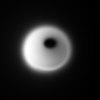
\includegraphics[width=.17\linewidth]
			{blackhole40.png} &
			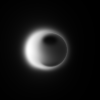
\includegraphics[width=.17\linewidth]
			{blackhole_orig.png} & 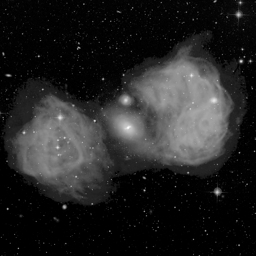
\includegraphics[width=.17\linewidth]
			{celestial-03-20.png} & 
			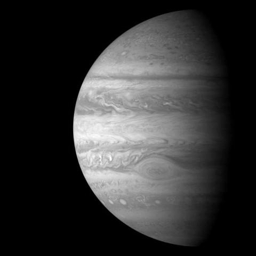
\includegraphics[width=.17\linewidth]
			{celestial-18-20.png}
			%\includegraphics[width=.15\linewidth]
			%{images/newfigs/results/celestial-03-30-6.png} 
			\\
			
			
			\hline
			&\vspace{-.1in}&&&\\
			\multirow{1}{*}[0.45in]{ \rotatebox[origin=t]{90}{{\textsf{Max Res}} }} &
			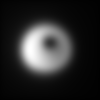
\includegraphics[width=.17\linewidth]
			{blackhole40_fliltered} &
			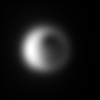
\includegraphics[width=.17\linewidth]
			{blackhole_filtered.png} & 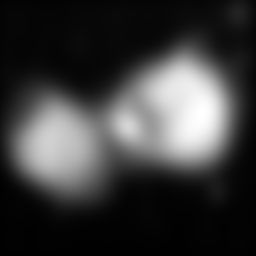
\includegraphics[width=.17\linewidth]
			{celestial-03-20-1.png} & 
			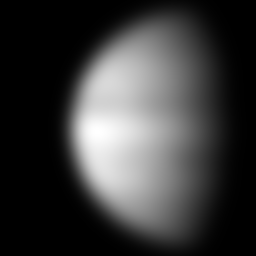
\includegraphics[width=.17\linewidth]
			{celestial-18-20-1.png}
			%\includegraphics[width=.15\linewidth]
			%{images/newfigs/results/celestial-03-10-6.png} 
			\\
			
			
		\end{tabular}
		\caption{ \footnotesize{{\bf Intrinsic Maximum Resolution:} The geometry of a telescope array imposes an intrinsic maximum resolution on the image you can reconstruct from the measurements. Recovering spatial frequencies higher than this resolution is equivalent to superresolution. For results presented, the minimum recoverable fringe spacing (corresponding to the maximum frequency) is 24.72 $\mu$-arcseconds. The original `Source' images (183.82 $\mu$-arcsecond FOV) are used to synthetically generate realistic VLBI measurements. We show the effect of filtering out spatial frequencies higher than the minimum fringe spacing for these source images in `Max Res'. }}
		\label{fig:maxres}
		\vspace{-.3in}
	\end{center}
\end{figure}



	\begin{figure*}[ht!]
		\vspace{-0.2in}
		\begin{center}
			\begin{tabular}{  c | c  c |  c  c  c  c | c  }
				%\hline
				
				
				& \multicolumn{2}{c}{ \small{\textsf{BLACK HOLE}} }  &   \multicolumn{4}{c}{ \small{\textsf{CELESTIAL}} } &  \small{\textsf{NATURAL}}  \\ \hline

				
				
				\vspace{-.1in} \cellcolor[gray]{0.8} & \cellcolor[gray]{0.8}& \cellcolor[gray]{0.8}& \cellcolor[gray]{0.8}& \cellcolor[gray]{0.8}&\cellcolor[gray]{0.8} & \cellcolor[gray]{0.8} & \cellcolor[gray]{0.8} \\
				
				\cellcolor[gray]{0.8} \multirow{1}{*}[.5in]{ \rotatebox[origin=t]{90}{{\textsf{TARGET}}} } &
				\cellcolor[gray]{0.8}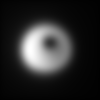
\includegraphics[width=.1\linewidth]
				{blackhole40_fliltered}  &
				\cellcolor[gray]{0.8}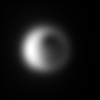
\includegraphics[width=.1\linewidth]
				{blackhole_filtered.png} &
				\cellcolor[gray]{0.8}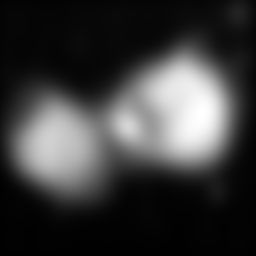
\includegraphics[width=.1\linewidth]
				{celestial-03-20-1.png} & \cellcolor[gray]{0.8}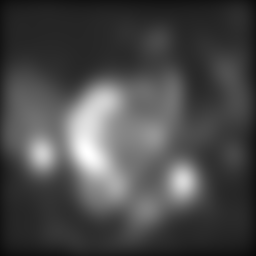
\includegraphics[width=.1\linewidth]
				{celestial-13-20-1.png}& \cellcolor[gray]{0.8}\cellcolor[gray]{0.8}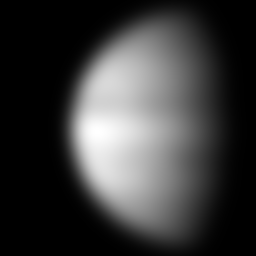
\includegraphics[width=.1\linewidth]
				{celestial-18-20-1.png}& \cellcolor[gray]{0.8}\cellcolor[gray]{0.8}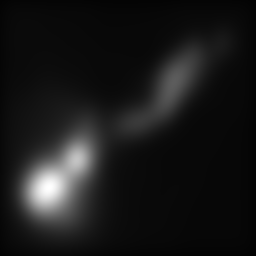
\includegraphics[width=.1\linewidth]
				{celestial-01-20-1.png}& \cellcolor[gray]{0.8}\cellcolor[gray]{0.8}
\includegraphics[width=.1\linewidth]
				{natural-03-20-1.png} \\
				\hline
				
			\vspace{-.1in}& &&&& & & \\
				
				\multirow{1}{*}[0.5in]{ \rotatebox[origin=t]{90}{{\textsf{CLEAN}}} } &
				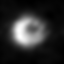
\includegraphics[width=.1\linewidth]
				{blackhole40_clean_1.png}  &
				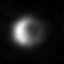
\includegraphics[width=.1\linewidth]
				{blackhole_clean_1.png} &
				
\includegraphics[width=.1\linewidth]
				{celestial_03_clean_1.png} & 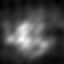
\includegraphics[width=.1\linewidth]
				{celestial_09_clean_1.png}& 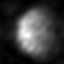
\includegraphics[width=.1\linewidth]
				{celestial_14_clean_1.png}& 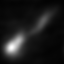
\includegraphics[width=.1\linewidth]
				{celestial_01_clean_1.png}& 
\includegraphics[width=.1\linewidth]
				{natural_03_clean_1.png} \\
				\hline
				
				\vspace{-.1in}& &&&& & & \\
				\multirow{1}{*}[0.55in]{ \rotatebox[origin=t]{90}{{\textsf{SQUEEZE}}} }&
				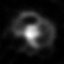
\includegraphics[width=.1\linewidth]
				{blackhole40_squeeze_1.png}  &
				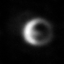
\includegraphics[width=.1\linewidth]
				{blackhole_1.png} &
				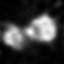
\includegraphics[width=.1\linewidth]
				{celestial_03_squeeze_1.png} & 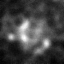
\includegraphics[width=.1\linewidth]
				{celestial_09_squeeze_1.png}& 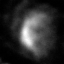
\includegraphics[width=.1\linewidth]
				{celestial_14_squeeze_1.png}& 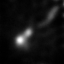
\includegraphics[width=.1\linewidth]
				{celestial_01_squeeze_1.png}& 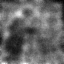
\includegraphics[width=.1\linewidth]
				{natural_03_squeeze_1.png} \\
				\hline
				
				\vspace{-.1in}& &&&& & & \\
				\multirow{1}{*}[0.5in]{ \rotatebox[origin=t]{90}{{\textsf{BSMEM}}} } &
				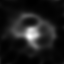
\includegraphics[width=.1\linewidth]
				{blackhole40_bsmem_1.png}  &
				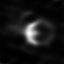
\includegraphics[width=.1\linewidth]
				{blackhole_bsmem_1.png} &
				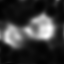
\includegraphics[width=.1\linewidth]
				{celestial_03_bsmem_1.png} & 
\includegraphics[width=.1\linewidth]
				{celestial_09_bsmem_1.png}& 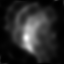
\includegraphics[width=.1\linewidth]
				{celestial_14_bsmem_1.png}& 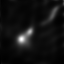
\includegraphics[width=.1\linewidth]
				{celestial_01_bsmem_1.png}& 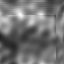
\includegraphics[width=.1\linewidth]
				{natural_03_bsmem_1.png} \\
				\hline
				
				\vspace{-.1in}\cellcolor[gray]{0.8} & \cellcolor[gray]{0.8}& \cellcolor[gray]{0.8}& \cellcolor[gray]{0.8}& \cellcolor[gray]{0.8}&\cellcolor[gray]{0.8} & \cellcolor[gray]{0.8} & \cellcolor[gray]{0.8} \\
				
				\cellcolor[gray]{0.8} \multirow{1}{*}[0.5in]{ \rotatebox[origin=t]{90}{{\textsf{CHIRP}}} } &
				\cellcolor[gray]{0.8}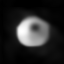
\includegraphics[width=.1\linewidth]
				{blackhole40_chirp_1_shift.png}  &
				\cellcolor[gray]{0.8}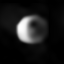
\includegraphics[width=.1\linewidth]
				{blackhole_chirp_1_shift.png} &
				\cellcolor[gray]{0.8}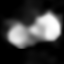
\includegraphics[width=.1\linewidth]
				{celestial_03_chirp_1_shift.png} & \cellcolor[gray]{0.8}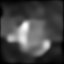
\includegraphics[width=.1\linewidth]
				{celestial_09_chirp_1.png}& \cellcolor[gray]{0.8}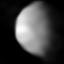
\includegraphics[width=.1\linewidth]
				{celestial_14_chirp_1.png}& \cellcolor[gray]{0.8}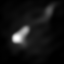
\includegraphics[width=.1\linewidth]
				{celestial_01_chirp_1.png}& \cellcolor[gray]{0.8}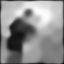
\includegraphics[width=.1\linewidth]
				{natural_03_chirp_1.png} \\
				\hline
\vspace{-.1in}& &&&& & & \\
				& \small{\textsf{A}}  & \small{\textsf{B}}  & \small{\textsf{C}}  & \small{\textsf{D}} & \small{\textsf{E}} & \small{\textsf{F}} &  \small{\textsf{G}}  \\ 
				
				
			\end{tabular}
			\caption{\footnotesize{ {\bf Method Comparison: } Comparison of our algorithm, `CHIRP' to three state-of-the-art methods: `CLEAN', `SQUEEZE', and `BSMEM'. We show the normalized reconstruction of a variety of black hole (a-b), celestial (c-f), and natural (g) source images with a total flux density (sum of pixel intensities) of 1 jansky and a 183.82 $\mu$-arcsecond FOV. Since absolute position is lost when using the bispectrum, shifts in the reconstructed source location are expected. The `TARGET' image shows the ground truth emission filtered to the maximum resolution intrinsic to this telescope array.  \vspace{-.2in}  
				}}
				\label{fig:comp}
			\end{center}
		\end{figure*}


	
	
	\begin{figure*}[t]
		\begin{center}
			\vspace{-.0in}
			\begin{tabular}{  c | c | c | c | c  }
				%\hline
				& \footnotesize{\textsf{CLEAN}}  & \footnotesize{\textsf{SQUEEZE}}  & \footnotesize{\textsf{BSMEM}} &  \cellcolor[gray]{0.8}\footnotesize{\textsf{CHIRP}}  \\ \hline
				&\vspace{-.1in}&&&\cellcolor[gray]{0.8}\\
				
				\multirow{1}{*}[0.4in]{ \rotatebox[origin=t]{90}{{\textsf{3.0 Flux}} }} &
				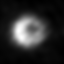
\includegraphics[width=.08\linewidth]
				{blackhole40_clean_3.png} &
				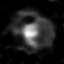
\includegraphics[width=.08\linewidth]
				{blackhole40_squeeze_3.png} & 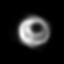
\includegraphics[width=.08\linewidth]
				{blackhole40_bsmem_3.png} & 
				\cellcolor[gray]{0.8}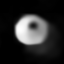
\includegraphics[width=.08\linewidth]
				{blackhole40_chirp_3_shift.png}
				%\includegraphics[width=.15\linewidth]
				%{images/newfigs/results/celestial-03-30-6.png} 
				\\
				
				
				\hline
				&\vspace{-.1in}&&&\cellcolor[gray]{0.8}\\
				\multirow{1}{*}[0.4in]{ \rotatebox[origin=t]{90}{{\textsf{2.0 Flux}} }} &
				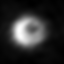
\includegraphics[width=.08\linewidth]
				{blackhole40_clean_2.png} &
				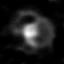
\includegraphics[width=.08\linewidth]
				{blackhole40_squeeze_2.png} & 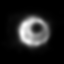
\includegraphics[width=.08\linewidth]
				{blackhole40_bsmem_2.png} & 
				\cellcolor[gray]{0.8}\includegraphics[width=.08\linewidth]
				{blackhole40_chirp_2_shift.png}
				%\includegraphics[width=.15\linewidth]
				%{images/newfigs/results/celestial-03-10-6.png} 
				\\
				
				
				\hline
				&\vspace{-.1in}&&&\cellcolor[gray]{0.8}\\
				\multirow{1}{*}[0.4in]{ \rotatebox[origin=t]{90}{{\textsf{0.5 Flux}} }} &
				\includegraphics[width=.08\linewidth]
				{blackhole40_clean_05.png} &
				\includegraphics[width=.08\linewidth]
				{blackhole40_squeeze_05.png} & \includegraphics[width=.08\linewidth]
				{blackhole40_bsmem_05.png} & 
				\cellcolor[gray]{0.8}\includegraphics[width=.08\linewidth]
				{blackhole40_chirp_05_shift.png}
				%\includegraphics[width=.15\linewidth]
				%{images/newfigs/results/celestial-03-05-6.png} 
				\\
				
				
				
				
				
				
			\end{tabular}
			\quad
			\begin{tabular}{  c | c | c | c | c  }
				%\hline
				& \footnotesize{\textsf{CLEAN}}  & \footnotesize{\textsf{SQUEEZE}}  & \footnotesize{\textsf{BSMEM}} &  \cellcolor[gray]{0.8}\footnotesize{\textsf{CHIRP}}  \\ \hline
				&\vspace{-.1in}&&&\cellcolor[gray]{0.8}\\
				
				\multirow{1}{*}[0.4in]{ \rotatebox[origin=t]{90}{{\textsf{3.0 Flux}} }} &
				\includegraphics[width=.08\linewidth]
				{celestial-03-30-3.png} &
				\includegraphics[width=.08\linewidth]
				{celestial_03_squeeze_flux3.png} & \includegraphics[width=.08\linewidth]
				{celestial_03_bsmem_3.png} & 
				\cellcolor[gray]{0.8}\includegraphics[width=.08\linewidth]
				{im4_chirp_flux3_shift.png}
				%\includegraphics[width=.15\linewidth]
				%{images/newfigs/results/celestial-03-30-6.png} 
				\\
				
				
				\hline
				&\vspace{-.1in}&&&\cellcolor[gray]{0.8}\\
				\multirow{1}{*}[0.4in]{ \rotatebox[origin=t]{90}{{\textsf{2.0 Flux}} }} &
				\includegraphics[width=.08\linewidth]
				{celestial-03-20-3.png} &
				\includegraphics[width=.08\linewidth]
				{celestial_03_squeeze_flux2.png} & \includegraphics[width=.08\linewidth]
				{celestial_03_bsmem_2.png} & 
				\cellcolor[gray]{0.8}\includegraphics[width=.08\linewidth]
				{im4_chirp_flux2_shift.png}
				%\includegraphics[width=.15\linewidth]
				%{images/newfigs/results/celestial-03-10-6.png} 
				\\
				
				
				\hline
				&\vspace{-.1in}&&&\cellcolor[gray]{0.8}\\
				\multirow{1}{*}[0.4in]{ \rotatebox[origin=t]{90}{{\textsf{0.5 Flux}} }} &
				\includegraphics[width=.08\linewidth]
				{celestial-03-05-3.png} &
				\includegraphics[width=.08\linewidth]
				{celestial_03_squeeze_flux05.png} & \includegraphics[width=.08\linewidth]
				{celestial_03_bsmem_05.png} & 
				\cellcolor[gray]{0.8}\includegraphics[width=.08\linewidth]
				{im4_chirp_flux05_shift.png}
				%\includegraphics[width=.15\linewidth]
				%{images/newfigs/results/celestial-03-05-6.png} 
				\\
				
				
				
				
				
				
			\end{tabular}
			\caption{ \footnotesize{{\bf Noise Sensitivity:} The effect of varying total flux density (in janskys), and thus noise, on each method's recovered reconstructions. Decreasing flux results in higher noise. Notice how our method is fairly robust to the noise, while the results from other methods often vary substantially across the noise levels. The ground truth target images along with the results for a total flux density of 1 jansky can been seen in column A and C of Figure~\ref{fig:comp}. 
					%Since absolute position is lost when using the bispectrum, shifts in the reconstructed source location are expected. 
					}}
			\label{fig:noise}
			\vspace{-.3in}
		\end{center}
	\end{figure*}
	


Measurements from the EHT have yet to become available.
% collected. 
Therefore, we demonstrate the success of our algorithm, CHIRP, on a sample of synthetic examples obtained from our online dataset and real VLBI measurements collected by the VLBA-BU-BLAZAR Program. 



\vspace{-.15in}
\paragraph{Synthetic Measurements}
For image results presented in the paper we generated synthetic data using realistic parameters for the EHT array pointed towards the black hole in M87.
Corresponding $(u,v)$ frequency coverage is shown in Figure~\ref{fig:uvcov}b.
%The minimum recoverable fringe spacing (corresponding to the maximum frequency) for this configuration is 24.72 $\mu$-arcseconds. 
The geometry of an array imposes an intrinsic maximum resolution on the image you can reconstruct from its measurements. Figure~\ref{fig:maxres} shows the effect of filtering out spatial frequencies higher than the minimum fringe spacing.
%{\it Recovering an image better than this filtered image is equivalent to performing superresolution.} 
These images set expectations on what is possible to reliably reconstruct from the measurements.
Additional results and details about the telescopes, noise properties, and parameter settings can be found in the supp. material~\cite{suppmaterial}. 

\vspace{-.15in}
\paragraph{Method Comparison} We compare results from our algorithm, CHIRP, with the three state-of-the-art algorithms described in Section~\ref{sec:related}: CLEAN, SQUEEZE, and BSMEM. 
%To eliminate bias, parameter choices for competing algorithms were discussed with their authors or knowlegeable users (provided in the supp. material)
%To eliminate bias, images were obtained by asking either the authors of the competing algorithms or knowledgeable users for reconstruction parameters (provided in the supp. material~\cite{suppmaterial}). 
Images were obtained by asking authors of the competing algorithms or knowledgeable users for a suggested set of reconstruction parameter (provided in the supp. material~\cite{suppmaterial}). 
The website submission system allows the results from other parameter settings and
algorithms to be compared, both qualitatively and quantitatively.
%Due to limited space, we only compared to some standard algorithms for sub-mm/mm VLBI. However, our online submission system allows the results of many different algorithms to be fairly compared, both qualitatively and quantitatively.


As with our algorithm, SQUEEZE~\cite{baron2010novel} and BSMEM~\cite{buscher1994direct} use the bispectrum as input. 
%For these methods we choose parameters that perform better than the expertly-chosen parameters used in~\cite{rusenimaging}.
CLEAN cannot automatically handle large phase errors, so CLEAN results were obtained using {\it calibrated} (eg. no atmospheric phase error) visibilities in CASA~\cite{jaeger2008common}. In reality, these ideal calibrated visibilities would not be available, and the phase would need to be recovered through highly user-dependent self-calibration methods. However, in the interest of a fair comparison, we show the results of CLEAN in a ``best-case" scenario. 

Figure~\ref{fig:comp} shows a sample of results comparing our reconstructions to those of the current state-of-the-art methods. Our algorithm is able to handle a wide variety of sources, ranging from very simple celestial to complex natural images, without any additional parameter tuning. 
%In most cases our method obtains superior results. 
CLEAN produces consistently blurrier results. %due to the final convolution with a reconstructing beam. 
%Although SQUEEZE should theoretically be able to obtain a global optimum for any cost function due to its MCMC framework, it is prohibitively complex and computationally expensive to exhaustively search all possibilities.
%Generally, BSMEM tends towards very sparse images. This strategy works well for super-resolution. %, such as in the second-to-last row of Figure~\ref{fig:comp}. 
Both SQUEEZE and BSMEM tend towards sparser images. This strategy works well for superresolution.
However, it comes at the cost of often making extended sources overly sparse and introducing spurious detail. 
%Our algorithm is able to handle a wide variety of sources without any additional parameter tuning. 
%To demonstrate reasonable results on natural images we have tuned SQUEEZE's parameters for the cameraman image in the last row.
Although algorithms such as BSMEM and SQUEEZE may perform better on these images with specific hand-tuned parameters, these tests demonstrate that the performance of CHIRP requires less user expertise and provides images that may be less sensitive to user bias.

Figure~\ref{fig:resultnums} shows a quantitative comparison of our method to SQUEEZE and BSMEM for the challenging, blind test set presented in Section~\ref{section:dataset}. 
%%In both metrics our method outperforms the current state-of-the-art algorithms. 
Since CLEAN cannot automatically handle large phase errors, we were unable to fairly compare its results on this test set. %Qualitative results with CLEAN assumed perfectly pre-calibrated data.  



\begin{figure}[t!]
		\vspace{-.25in}
	\centering
	\subfigure{\includegraphics[width=0.49\linewidth]
		{blinddataset/mse.pdf}}
	\subfigure{\includegraphics[width=0.49\linewidth]
		{blinddataset/ssim.pdf}}
	\caption{\footnotesize{ {\bf Quantitative Analysis on Blind Test Set:}  Box plots of MSE and SSIM for reconstruction methods on the blind dataset presented in Section~\ref{section:dataset}. 
			%We believe better error metrics for this application should be subject for future research. 
			%Although, our method outperforms SQUEEZE and BSMEM under these metrics, we believe better error metrics for this application should be subject for future research. 
			In SSIM a score of 1 implies perceptual indistinguishability between the ground truth and recovered image. Scores are calculated using the original `Source' image (Refer to Fig.~\ref{fig:maxres}). 
			%SSIM returns a score between -1 and +1, where +1 implies that the two images are perceptually indistinguishable. 
			%Images were automatically aligned and normalized before each error metric was computed. 
		}}
	\label{fig:resultnums}
	\vspace{-0.23in}
\end{figure}


%\begin{table}
%	\begin{center}
%		%\vspace{-0.2in}
%		\begin{tabular}{ | c | c |c | c|  }
%			\hline
%			& \footnotesize{\textsf{SQUEEZE}} & \footnotesize{\textsf{BSMEM}} & \cellcolor[gray]{0.8}\footnotesize{\textsf{CHIRP}}   \\ \hline 
%			
%			{\footnotesize{\textsf{MSE}}}& \footnotesize{{0.0308 $\pm$ 0.0431 }} & \footnotesize{{0.0242 $\pm$ 0.0310}} & \cellcolor[gray]{0.8}{ \footnotesize{{0.0199 $\pm$ 0.0345 }} }  \\ \hline
%			
%			{\small{\textsf{SSIM}}}& \footnotesize{{0.9409 $\pm$ 0.0375}} & \footnotesize{{0.9405 $\pm$ 0.0347}} & \cellcolor[gray]{0.8}{ \footnotesize{{0.9424 $\pm$ 0.0199}} }  \\ \hline
%			
%		\end{tabular}
%		\vspace{.05in} 
%		\caption{\footnotesize{ {\bf Quantitative Analysis on Blind Test Set}  MSE and SSIM scores (mean $\pm$ standard deviation) for reconstruction methods on the blind dataset presented in Section~\ref{section:dataset}. Large standard deviation values are due to outliers. We believe better error metrics for this application should be subject for future research. 
		%Although, our method outperforms SQUEEZE and BSMEM under these metrics, we believe better error metrics for this application should be subject for future research. 
%				In SSIM a score of 1 implies perceptual indisguisability between the groundtruth and recovered image. Scores are calculated using the original 'Source' image (Refer to Fig.~\ref{fig:maxres}). 
%				%SSIM returns a score between -1 and +1, where +1 implies that the two images are perceptually indistinguishable. 
%				%Images were automatically aligned and normalized before each error metric was computed. 
%			}}
%			\label{table:resultnums}
%			\vspace{-.3in}
%		\end{center}
%	\end{table}


\vspace{-.15in}
\paragraph{Noise Sensitivity} The standard deviation of thermal noise introduced in each measured visibility is fixed based on measurement choices and the corresponding telescopes' properties. Specifically, $\sigma = \frac{1}{0.88} \sqrt{ {\rho_1 \rho_2 }/{ \nu T } } $ for bandwidth $\nu$, integration time $T$, and each telescope's System Equivalent Flux Density ($\rho$).
%\footnote{The $\frac{1}{0.88}$ factor is due to quantization in the A/D converter CITATION}.
Consequently, an emission with a lower total flux will result in a lower SNR signal.


Previous measurements predict that the total flux densities of the black holes M87 and SgA* will be in the range 0.5 to 3.0 janskys
% (total intensity of the source image)
~\cite{doeleman2012jet, doeleman2008event}.
Figure~\ref{fig:noise} shows the effect of varying total flux density, and thus noise, on each method's recovered reconstructions. Notice how our method is fairly robust to the noise, while the results from other methods often vary substantially across noise levels. 





%\vspace{-0.1in}
%\paragraph{Mitigation of Scattering}

%In Section BLAH we discuss inverting the blurring effect caused by interstellar scattering while simultaneously reconstructing an image from the bispectrum measurements. The interestellar scattering introduced in the path to black hole SgA* is described by a Gaussian with covariance (radians)

%\begin{equation}
%\Sigma = \Spvek{ 2.00614 \times 10^{-21} \hspace{0.2in} %3.21018 \times 10^{-22}; 3.21018 \times 10^{-22} %\hspace{0.2in} 5.64104 \times 10^{-22}}
%\end{equation}

%Figure~\ref{fig:scattering} shows the effect of this scattering kernel on the ideal image and maximum resolution recoverable image. 
%Inverting scattering before (by dividing visibilities) or after imaging results in a sub-optimal image containing artifacts (Refer to Figures BLAH).
%However, by introducing this blurring into our forward model, and thus the energy's data term, we avoid introducing false information, and produce a more realiable, ''sharp" image.
%The sharpness of our result is comparable to that of an image recovered when scattering is not incoperated in the simulated visibility measurements. 



%\vspace{-0.1in}
%\paragraph{Effect of Prior Model} In Section BLAH we introduced the idea of using different patch models to reconstruct an image. We demostrate this idea by using 3 different sets of images with distinct statistics to train a patch prior model: natural, celestial, and simulated images of a black hole. 
%Figure BLAH shows the effect of using each patch model on the resulting reconstructed image. 
%Although small variations can be observed between the images, it does not lead to large differences. 
%This suggests that with our selected parameters, the prior helps in guiding the optimization, but does not impose strong assumptions that may bias our results.   
%Perhaps more intersting is the 
 
% \begin{figure}[b]
% 	\begin{center}
% 		\vspace{-.2in}
% 		\begin{tabular}{c c c c c}
% 			%\hline
% 			\small{\textsf{}}  & \hspace{-.17in} \small{\textsf{}}  & \hspace{-.17in}
% 			\small{\textsf{Natural}}  & \hspace{-.17in} \small{\textsf{Celestial}}  & \hspace{-.17in} \small{\textsf{Black Hole}} \\
% 			
% 			\small{\textsf{Source}}  & \hspace{-.17in} \small{\textsf{Filtered}}  & \hspace{-.17in}
% 			\small{\textsf{Prior}}  & \hspace{-.17in} \small{\textsf{Prior}}  & \hspace{-.17in} \small{\textsf{ Prior}} \\
% 			
% 			
% 			\includegraphics[width=.19\linewidth]
% 			{images/newfigs/prior/orig.png} & 	\hspace{-.17in}
% 			\includegraphics[width=.19\linewidth]
% 			{images/newfigs/prior/beamed.png} & 	\hspace{-.17in}
% 			\includegraphics[width=.19\linewidth]
% 			{images/newfigs/prior/pmap_bs_055_050_2_natural_2000_halffov.png} & 	\hspace{-.17in} \includegraphics[width=.19\linewidth]
% 			{images/newfigs/prior/pmap_bs_055_050_2_celestial_2000_halffov.png} & 	\hspace{-.17in}
% 			\includegraphics[width=.19\linewidth]
% 			{images/newfigs/prior/pmap_bs_055_050_2_blackhole_2000_halffov.png} \\
% 			
% 			
% 			
% 		\end{tabular}
% 		\caption{ \footnotesize{{\bf Effect of Patch Prior:} Reconstructions of a 128.67 $\mu$-arcsecond FOV using patch priors trained on natural, celestial, and synthetic black hole images. Although the underlying statistics of these images are very different, the common dominant low frequency patches drive optimization, resulting in very similar reconstructions. }}
% 		\label{fig:patchprior}
% 		\vspace{-.35in}
% 	\end{center}
% \end{figure}
% 
 
 
 
 
 
 
 \begin{figure}[b]
 	\begin{center}
 		\vspace{-.2in}
 		
% 		
% 		\begin{tabular}{c c}
% 			
% 			
% 			\small{\textsf{Source}}  & \hspace{-.17in} \small{\textsf{Filtered}}  \\
% 			
% 			
% 			\includegraphics[width=.19\linewidth]
% 			{images/newfigs/prior/orig.png}  &	\hspace{-.17in}
% 			\includegraphics[width=.19\linewidth]
% 			{images/newfigs/prior/beamed.png} 	\hspace{-.17in} \\
% 			
% 			
% 			
% 		\end{tabular}
 		
 		
 		
 		
 		\begin{tabular}{c c c c c}
 			%\hline
 			
 			
 			\includegraphics[width=.19\linewidth]
 			{blackhole_chirp_1_shift.png} & 	\hspace{-.17in} \includegraphics[width=.19\linewidth]
 			{blackhole_celestial_shift.png} & 	\hspace{-.17in}
 			\includegraphics[width=.19\linewidth]
 			{blackhole_blackhole_shift.png}& 	\hspace{-.17in}
 			\includegraphics[width=.19\linewidth]
 			{blackhole_l2.png}& 	\hspace{-.17in} 
 			\includegraphics[width=.19\linewidth]
 			{blackhole_l08_lambda200.png} \\
 			
 			
 			 			\includegraphics[width=.19\linewidth]
 			 			{celestial_14_chirp_1.png} & 	\hspace{-.17in} \includegraphics[width=.19\linewidth]
 			 			{celestial_14_celestial.png} & 	\hspace{-.17in}
 			 			\includegraphics[width=.19\linewidth]
 			 			{celestial_14_blackhole.png}& 	\hspace{-.17in}
 			 			\includegraphics[width=.19\linewidth]
 			 			{celestial14_l2.png}& 	\hspace{-.17in} 
 			 			\includegraphics[width=.19\linewidth]
 			 			{celestial14_l08.png} \\
 			
 			\small{\textsf{Natural}}  & \hspace{-.17in} \small{\textsf{Celestial}}  & \hspace{-.17in}
 			\small{\textsf{Black Hole}}  & \hspace{-.17in} \small{\textsf{$\ell_2$ Norm}}  & \hspace{-.17in} \small{\textsf{$\ell_{0.8}$ Norm}} \\
 			
 			%	\footnotesize{\textsf{Patch Prior}}  & \hspace{-.17in} \footnotesize{\textsf{Patch Prior}}  & \hspace{-.17in}
 			%	\footnotesize{\textsf{Patch Prior}}  & \hspace{-.17in} \footnotesize{\textsf{Prior}}  & \hspace{-.17in} \footnotesize{\textsf{ Prior}} \\
 			
 			
 			
 		\end{tabular}
 		\caption{ \footnotesize{{\bf Effect of Patch Prior:} Reconstructions using patch priors trained on natural, celestial, and synthetic black hole images as well as $\ell_2$ and $\ell_{0.8}$ norm priors on the residuals. The ground truth target image are shown in Figure~\ref{fig:comp} column B and E. 
 				%Although the underlying statistics of natural, celestial, and black hole images are very different,
 				%their common dominant low frequency patches drive optimization, resulting in very similar reconstructions. 
 				The patch priors outperform results obtained using simpler $\ell$-norm priors. 
 				Since absolute position is lost during imaging, shifts in the reconstructed source location are expected. 
 				} }
 		\label{fig:patchprior}
 		\vspace{-.35in}
 	\end{center}
 \end{figure}
 
 
 
 
 
 \vspace{-.15in}
 \paragraph{Effect of Patch Prior} Flexibility of the patch prior framework allows us to easily incorporate a variety of different ``visual" assumptions in our reconstructed image.
 %on what we expect to see in $I_{\lambda}$. 
 For instance, in the case of the EHT, simulations of a black hole for different inclinations and spins can be used to train a patch model that can be subsequently used for reconstruction. 
 %Although this may bias results, reconstrucing under a number of different priors presents a range of solutions that vary from weak assumptions with high variance to strong assumptions with low variance. 
 In Figure~\ref{fig:patchprior} we show results using a patch prior trained on natural~\cite{martin2001database}, celestial, and synthetic black hole images%(with varying inclination and spin)
 ~\cite{avery}. Only small variations can be observed among the resulting images.
 Given our selected parameters, this suggests that the prior guides optimization, but does not impose strong assumptions that may greatly bias results.
  
 %demonstrate performance
 
 
\vspace{-.2in}
\paragraph{Real Measurements} 

We demonstrate the performance of our algorithm on the reconstruction of three different sources using real VLBI data from
%the VLBA-BU-BLAZAR Program
~\cite{jorstad2005polarimetric} in Figure~\ref{fig:realdata}.
Although we do not have ground truth images corresponding to these measurements, we compare our reconstructions to those generated by the BU group,
reconstructed using an interactive calibration procedure described in~\cite{jorstad2005polarimetric}.
%These images were reconstructed using a complex and time-consuming procedure of self-calibration described in~\cite{jorstad2005polarimetric}. 
Alternatively, we are able to use bispectrum measurements to automatically produce image reconstructions with minimal user input. Notice that we are able to recover sharper images, and even resolve two potentially distinct sources that were previously unresolved in blazar OJ287. 


%Thee published blazar data has been phase calibrated using a combination of CLEAN self-calibration and observation of calibration sources. Although the data has been calibrated, this calibration is ignored when using the bispectrum. Therefore, we are able to fairly evaluate how well we would preform on uncalibrated data.  



\begin{figure}[tb]
	\begin{center}
		\vspace{-.25in}
		\begin{tabular}{  c | c | c | c   }
			%\hline
			&  \small{\textsf{3C279}}  & \small{\textsf{OJ287}}  & \small{\textsf{BL Lacertae}}   \\ \hline
			&\vspace{-.1in}&&\\
			\multirow{1}{*}[0.6in]{ \rotatebox[origin=t]{90}{{\textsf{BU Results}} }}& 
			\includegraphics[width=.2\linewidth]
			{3C279NOV13_gt.png} &
			\includegraphics[width=.2\linewidth]
			{OJ287Aug10B_gt.png} &
			\includegraphics[width=.2\linewidth]
			{BLLACAPR10D_gt.png}  \\
			
			\hline
			
			&\vspace{-.1in}&&\\
			\multirow{1}{*}[0.5in]{ \rotatebox[origin=t]{90}{{\textsf{CHIRP}} }}& 
			\includegraphics[width=.2\linewidth]
			{3C279NOV13_mine.png} &
			\includegraphics[width=.2\linewidth]
			{OJ287Aug10B_mine.png} &
			\includegraphics[width=.2\linewidth]
			{BLLACAPR10D_mine.png}  \\
			
			
		\end{tabular}
		\caption{ \footnotesize{{\bf Real Measurements:} A comparison of our reconstructed images to~\cite{jorstad2005polarimetric}'s results using CLEAN self-calibration. Note that we are able to reconstruct less blurry images, and are even able to resolve 2 separate, previously unresolved, bright emissions in blazar OJ287. Measurements were taken using the VLBA telescope array. The FOV for each image is 1.5, 1, and 1 milli-arcsecond respectively.} }
		\label{fig:realdata}
		\vspace{-.3in}
	\end{center}
\end{figure}


\vspace{-.1in}
\section{Conclusion}
\vspace{-.1in}
Astronomical imaging will benefit from the cross-fertilization of ideas with the computer vision community. 
%By bridging the gap between astronomy and computer vision, our work initiates the transfer of ideas developed in computer vision to applications in VLBI.
In this paper, we have presented an algorithm, CHIRP, for reconstructing an image using a very sparse number of VLBI frequency constraints.
We have demonstrated improved performance compared to current state-of-the-art methods on both synthetic and real data.
Furthermore, we have introduced a new dataset for the testing and
development of new reconstruction algorithms.  
With this paper, the
dataset, and algorithm comparison website, we hope to make this
problem accessible to researchers in computer vision, and push the limits of celestial imaging. 

%With this paper, the
%dataset, and algorithm comparison web page, we hope to make this
%problem accessible to researchers in the computer vision community.
%By introducing a new dataset to aid in the testing and development of new reconstruction algorithms, we hope to make this problem accessible to researchers in the computer vision community. 
%Recently, high resolution VLBI imaging has helped to uncover many new high-impact findings~\cite{deane2014close}. We hope that pushing the limits of celestial imaging will result in exciting future discoveries. 


\vspace{-0.04in}
\footnotesize{
\paragraph{Acknowledgments}

We would like to thank Andrew Chael, Katherine Rosenfeld, Lindy Blackburn, and Fabien Baron for all of their helpful discussions and feedback. 
This work was partially supported by NSF CGV-1111415.
Katherine Bouman was partially supported by an NSF Graduate Fellowship.
We also thank the National Science Foundation (AST-1310896, AST-1211539, and AST-1440254) and the Gordon and Betty Moore Foundation (GBMF-3561) for financial support of this work.
This study makes use of 43 GHz VLBA data from the VLBA-BU Blazar Monitoring Program (VLBA-BU-BLAZAR;
http://www.bu.edu/blazars/VLBAproject.html), funded by NASA through the Fermi Guest Investigator Program. The VLBA is an instrument of the National Radio Astronomy Observatory. The National Radio Astronomy Observatory is a facility of the National Science Foundation operated by Associated Universities, Inc.
}



%\katie{ (Doeleman et al, Nature, v455, p.78, 2008; Doeleman et al, Science, v338, p.355, 2012; Fish et al, ApJL, v.727, p.36, 2011).reference for closure phase and bispectrum : Rogers, Doeleman  Moran, AJ, v. 109, p.1391, (1995).
	}
